\chapter{Results and Interpretation}

Through the extensive procedures outlined in the previous chapter, a set of final results can be provided. Here, the event distributions versus $M_{\gamma^*}, x_F, p_T, x_1,$ and $\cos\theta$ are presented. Finally, the per-nucleon cross section ratios are shown for \emph{C/D}, \emph{Fe/D}, and \emph{W/D}, along with an interpretation of these ratios with respect to nuclear $x-$scaling.

\section{Drell-Yan Event Distributions}

The following kinematic distributions represent the acceptance of the SeaQuest dimuon spectrometer. By measuring the momenta ($p_{\mu}$) of the muon tracks at the vertex position, the quantities of invariant mass ($M_{\gamma^*}$), $x_F$, and $p_T$ of the virtual photon can be calculated.
\begin{eqnarray}
p_\mu & = & (p_x, p_y, p_z) \\
E_{\mu^+\mu^-} & = & \sqrt{|p_{\mu^+}|^2 + |p_{\mu^-}|^2} \\
P_{\mu^+\mu^-} & = & p_{\mu^+} + p_{\mu^-} \\
p_T & = & \sqrt{(p_{\mu^+}^x + p_{\mu^+}^x)^2 + (p_{\mu^+}^y + p_{\mu^+}^y )^2} \\
p_z & = & p_{\mu^+}^z + p_{\mu^+}^z \\
M_{\gamma^*} & = & \sqrt{E_{\mu^+\mu^-}^2 - P_{\mu^+\mu^-}^2} \\
x_F & = & \frac{p_{\mu^+}^z + p_{\mu^+}^z }{\sqrt{s}/2 (1-M^2_{\gamma^*}/s)} \rightarrow 2(p_{\mu^+}^z + p_{\mu^+}^z)/\sqrt{s} \\
\end{eqnarray}
From these, $x_1$ and $x_2$ can be derived according to Eqs.~\ref{eq:x1-x2-tau}.

The distributions of the dimuon kinematic quantities $x_F, M_{\gamma^*}, p_T$, and $p_z$ can be found in Figure~\ref{fig:event-dist1} while the quark quantities $x_1, x_2,$ and $\cos\theta_\mu$ can be found in Figure~\ref{fig:event-dist2}. As can be seen from the distributions, the SeaQuest experiment studies muons with an invariant mass between 4.2 and \unit[10]{GeV} (the range between the $\phi^\prime$ and the $\upsilon$), and the acceptance measures mostly forward-moving ($x_F>0$) muon pairs with longitudinal momentum ($p_z$) greater than \unit[40]{GeV} in the lab frame. The acceptance of $p_T$ of the muon pair is limited to \unit[3]{GeV}. It is worth noting that, as can be seen from the $\cos\theta_\mu$ distribution, there is certainly contamination evident at the tails of the distribution, primarily in the positive $\cos\theta$ region. This is one of the key clues that SeaQuest has a problem with \emph{combinatoric} background, or reconstructed muon pairs that arise from uncorrelated muons produced in the target or beam dump.

The beam quarks participating in the Drell-Yan process can have a fractional momentum $x_1$ ranging from around 0.35 to 0.9 with the distribution peaking at 0.57 and having a mean value of $\langle x_1 \rangle = 0.6$, and the target antiquark participating in the interaction can possess a fractional momentum $x_2$ ranging from 0.1 to 0.5, with the distribution peaking at around 0.16 and having a mean value of $\langle x_2 \rangle = 0.2$. A table of the total mean kinematics and also the mean kinematics for each $x_2$ bin can be found in Table~\ref{tab:mean-kin-x2}.

\begin{figure}
	\centering
	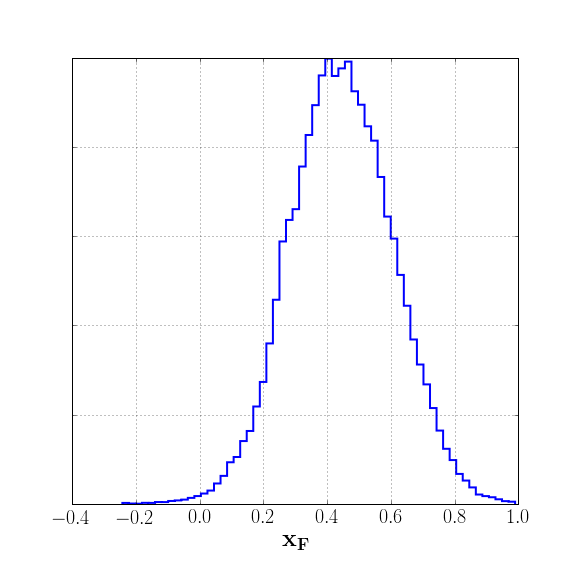
\includegraphics[width=0.48\textwidth]{figures/results/xF-dist.png} \hfill
	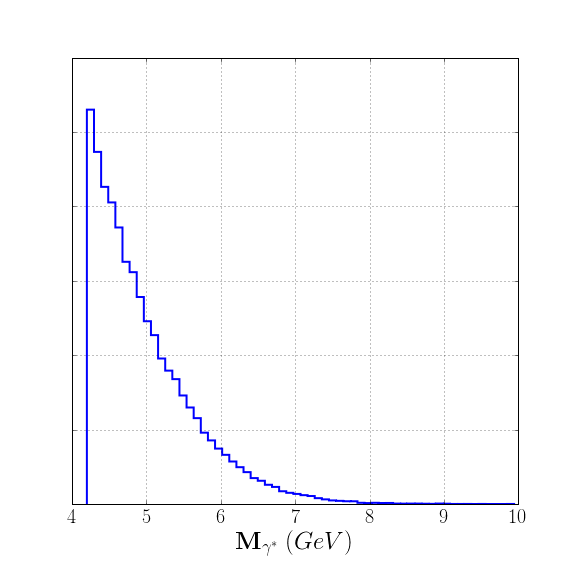
\includegraphics[width=0.48\textwidth]{figures/results/mass-dist.png}	
	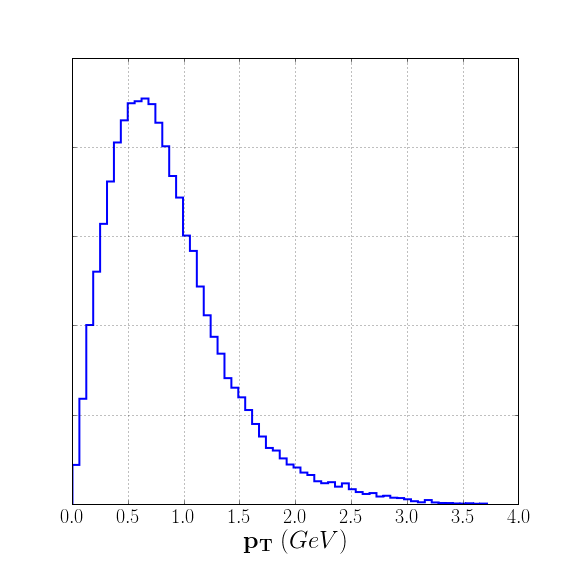
\includegraphics[width=0.48\textwidth]{figures/results/pt-dist.png} \hfill
	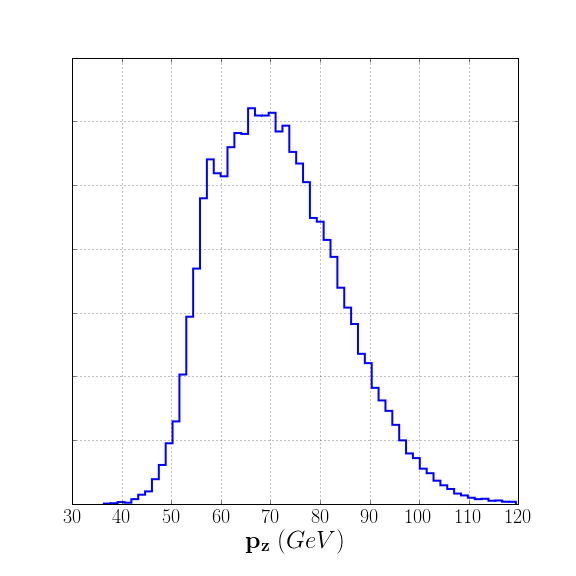
\includegraphics[width=0.48\textwidth]{figures/results/pz-dist.png} \\
	\caption{Event distributions for all combined data versus dimuon kinematic variables $x_F, M_{\gamma^*}, p_T,$ and $p_z$}
	\label{fig:event-dist1}
\end{figure}

\begin{figure}
	\centering
	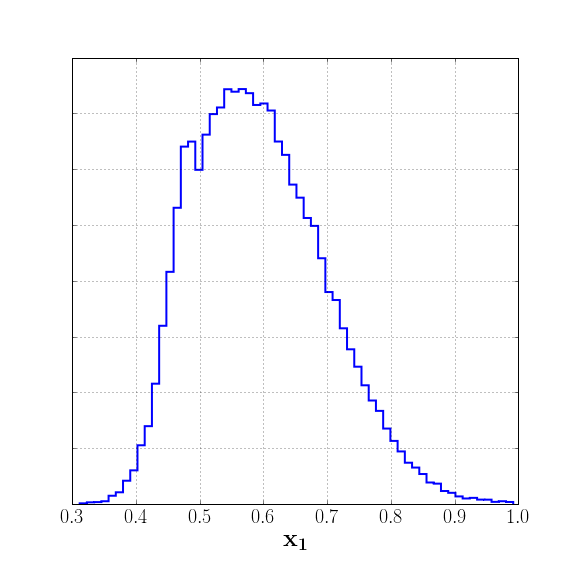
\includegraphics[width=0.48\textwidth]{figures/results/x1-dist.png} \hfill
	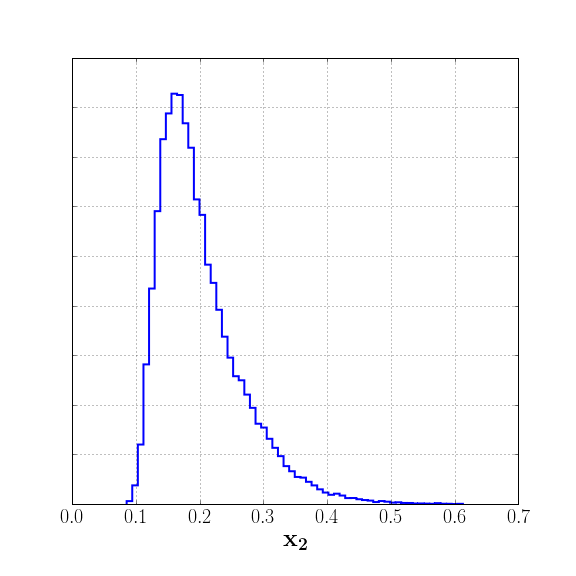
\includegraphics[width=0.48\textwidth]{figures/results/x2-dist.png} \\
	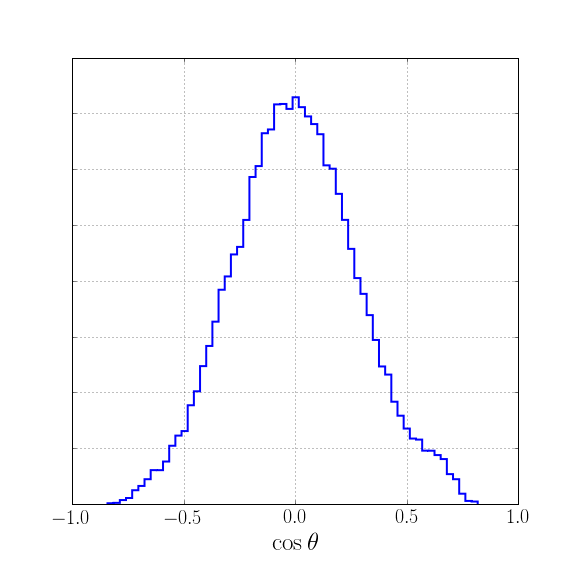
\includegraphics[width=0.48\textwidth]{figures/results/costh-dist.png}
	\caption{Event distributions for all combined data versus quark kinematic variables $x_1, x_2,$ and the cosine of the polar decay angle, $\theta_\mu$}
	\label{fig:event-dist2}
\end{figure}

\begin{sidewaystable}
	\centering
	\ra{1.3}
	\begin{tabular}{lrrrrrrrrrrrr}
		\toprule
		{} &    $\langle x_1 \rangle$ &    $\langle x_2\rangle$ &   $\langle M_{\gamma^*}\rangle$ &     $\langle x_F\rangle$ &  $\langle \cos\theta_\mu\rangle$ &    $\langle \phi_\mu\rangle$ &     $\langle p_z\rangle$ &    $\langle p_T\rangle$ &     $\langle p_z^+\rangle$ &    $\langle p_z^-\rangle$  &    $\langle p_T^+\rangle$ &   $\langle p_T^-\rangle$  \\
		$x_2$-bin            &        &        &   (GeV)     &        &        &        &     (GeV)    &   (GeV)     &    (GeV)     &   (GeV)      &   (GeV)     &   (GeV)     \\
		\midrule
		(0.1, 0.13]   &  0.746 &  0.120 &  4.378 &  0.690 &  0.011 &  0.043 &  90.145 &  0.737 &  45.815 &  44.329 &  2.124 &  2.112 \\
		\rowcol (0.13, 0.16]  &  0.650 &  0.146 &  4.516 &  0.559 & -0.005 & -0.030 &  78.487 &  0.762 &  39.415 &  39.079 &  2.224 &  2.186 \\
		(0.16, 0.195] &  0.592 &  0.177 &  4.751 &  0.467 & -0.011 & -0.008 &  71.473 &  0.805 &  35.833 &  35.641 &  2.365 &  2.305 \\
		\rowcol (0.195, 0.24] &  0.567 &  0.215 &  5.143 &  0.404 & -0.009 &  0.008 &  68.394 &  0.841 &  34.344 &  34.015 &  2.562 &  2.500 \\
		(0.24, 0.29]  &  0.557 &  0.262 &  5.626 &  0.348 & -0.007 &  0.008 &  67.097 &  0.900 &  33.728 &  33.349 &  2.800 &  2.726 \\
		\rowcol (0.29, 0.35]  &  0.543 &  0.314 &  6.079 &  0.280 & -0.021 &  0.038 &  65.423 &  1.008 &  32.313 &  33.088 &  3.013 &  2.941 \\
		(0.35, 0.45]  &  0.535 &  0.386 &  6.713 &  0.191 & -0.005 &  0.024 &  64.301 &  0.994 &  32.014 &  32.282 &  3.319 &  3.304 \\
		\rowcol (0.45, 0.58]  &  0.512 &  0.485 &  7.331 &  0.040 & -0.019 & -0.220 &  61.508 &  1.086 &  31.295 &  30.323 &  3.715 &  3.626 \\
		\bottomrule
		\textbf{Combined:} & 0.601 &  0.201 &  5.012 &  0.453 & -0.002 & 0.000 & 72.553 &  0.865 &  36.444 &  36.109 &  2.472 & 2.441 \\
	\end{tabular}
	\caption{The mean dimuon kinematics in each bin of $x_2$. These should be considered to be appro/ximate, as they are
		calculated as a weighted average from the data set when corrected for rate dependence in $x_2$.}
	\label{tab:mean-kin-x2}
\end{sidewaystable}


\section{Nuclear x-Scaling}

When discussing heavy nuclei and, a certain shift in understanding of scaling variables should be considered. The use of the Bjorken-$x$ scaling variable up until now should be noted to be the parton momentum fraction \emph{of the proton} $x_p = Q^2/(2 m_p \omega)$. It has been recently discussed by Frankfurt \& Strikman\cite{Frankfurt:2012qs} and implemented by Hen \emph{et al.}\cite{Hen:2013oha} that the \emph{structure functions of nucleons bound in nuclei should be extracted in the reference frame of the nucleus}. This is done by considering to the $x_A$ scaling variable, defined as:
\begin{equation}
\frac{x_A}{A} = \frac{Q^2}{2q\cdot P_A} \ \ \ ;\ \ \ x_A = \frac{Q^2}{2q\cdot P_A/A} = \frac{AQ^2}{2\omega m_A} = x_p \cdot \frac{A m_p}{m_A}
\end{equation}
where $q$ and $P_A$ are the 4-momentum vectors of the virtual photon and target nucleus respectively, and $m_A$ is the mass of the target nucleus. For the same values of $Q^2$ and $\omega$, $x_A$ differs from $x_p$ by the ratio of the bound nucleon mass to the free mass. Therefore, a cross section measured at $Q^2$ and $\omega$ on a nucleus $A$ will depend on the nucleon structure function evaluated at $x_A$ rather than $x_p$. For converting from the commonly used $x_p$ over to $x_A$ for the different targets, we apply a factor of $\frac{A m_p}{m_A}$, which for deuterium, carbon, iron, and tungsten are AAAAA, BBBBB, CCCCC, and DDDDD, respectively.

As a result, this means that the standard EMC cross section ratio is actually proportional to the nucleon structure function in nucleus $A$ evaluated at parton momentum $x_A$ divided by the nucleon structure function in deuterium evaluated at parton momentum fraction $x_D$ ($x_D = 2Q^2/2m_D\omega = x_p \cdot 2m_p/m_D$)\cite{Hen:2013oha}. For a symmetric nuclei, this can be written as:
\begin{equation}
\frac{2}{A} \cdot \frac{\sigma^A_{DY}(x_p, Q^2)}{\sigma^D_{DY}(x_p, Q^2)} = \frac{F_2^A(x_A, Q^2)}{F_2^D(x_D, Q^2)}
\end{equation}
where $\frac{F_2^A(x_A, Q^2)}{F_2^D(x_D, Q^2)}$ is the ratio of structure functions at the same $Q^2$, but at different $x$. Since we want to compare the structure functions at the same parton momentum fractions, we correct this by using
\begin{eqnarray}
\frac{F_2^A(x_A, Q^2)}{F_2^D(x_D, Q^2)} & = & \frac{F_2^A(x_A, Q^2)}{F_2^D(x_A, Q^2)} \cdot \frac{F_2^D(x_A, Q^2)}{F_2^D(x_D, Q^2)} \\
& & \nonumber \\
\frac{F_2^A(x_A, Q^2)}{F_2^D(x_A, Q^2)} & = & \frac{2}{A} \cdot \frac{\sigma^A_{DY}(x_p, Q^2)}{\sigma^D_{DY}(x_p, Q^2)} \cdot \frac{F_2^D(x_D, Q^2)}{F_2^D(x_A, Q^2)}
\label{eq:struc-func-ratio-xA}
\end{eqnarray}
where here we have $\frac{F_2^D(x_D, Q^2)}{F_2^D(x_A, Q^2)}$ as a correction factor to arrive at $\frac{F_2^A(x_A, Q^2)}{F_2^D(x_A, Q^2)}$, which is the ratio of structure functions in the different nuclei evaluated at the same parton momentum fraction (which is what we're looking to extract). The correction factor can be evaluated using well-known parameterizations of the the structure function of the deuteron~\cite{Whitlow:1991uw,Bosted:2007xd}. In \red{Figure~refAAA}, the correction factor $\frac{F_2^D(x_D, Q^2)}{F_2^D(x_A, Q^2)}$ is shown as a function of $x_p$ for different targets.

In summary, the traditional EMC per-nucleon cross section ratio measurement has yielded a ratio for $\frac{F_2^A(x_A)}{F_2^D(x_D)}$, when what is really desired is $\frac{F_2^A(x_A)}{F_2^D(x_A)}$. The addition of this $\frac{F_2^D(x_D)}{F_2^D(x_A)}$ correction factor is all that is needed to convert the measurement to the desired result. This correction factor will be applied to the SeaQuest result.
